\section{Problem formulation}\label{sec:problem}

We consider a single worker who processes a stream of tasks during one workday. A scheduler, which could be a digital assistant, a workflow-management system or a supervisory controller in a human--robot cell, decides at regular intervals what the worker should do next: start or continue an easy task, a hard task, or take a short break. The worker's capacity depends on a latent cognitive state that evolves with the schedule. Table~\ref{tab:notation} summarises the notation and Table~\ref{tab:params} lists the parameter values.

\begin{table}[t]
\centering
\caption{Notation.}
\label{tab:notation}
\small
\begin{tabular}{ll}
\toprule
Symbol & Meaning \\
\midrule
$t\in\{0,\dots,T-1\}$, $\Delta$ & decision slot index and slot length ($T=48$, $\Delta=10$ min) \\
$h_t$ & clock time of slot $t$ (h), $h_t=9+t\Delta/60$ \\
$a_i, d_i, w_i, D_i$ & arrival slot, difficulty, work content and deadline of task $i$ \\
$H_t$ & homeostatic attention resource (latent) \\
$c(h)$, $A_t$ & circadian modulation and effective attention, $A_t=\mathrm{clip}(H_t+\gamma c(h_t))$ \\
$F_t$ & fatigue (latent) \\
$\rho_t$ & work rate (work units completed per slot) \\
$\tilde A_t,\tilde F_t$ & noisy observations of $A_t,F_t$ \\
$o_t$, $x_t$ & observation vector and history window of length $k$ \\
$u_t, b_t$ & indicators of working and resting in slot $t$ \\
$r_t$ & scalar reward; $\lambda,\mu$ fatigue and attention weights \\
$\gamma_{\mathrm{RL}}$ & RL discount factor (distinct from circadian amplitude $\gamma$) \\
\bottomrule
\end{tabular}
\end{table}

\subsection{Workload model}
The day is divided into $T=48$ slots of $\Delta=10$ minutes (09:00--17:00). Each day contains $N=12$ tasks. Six tasks are available at the start of the day and the remaining six arrive at slots drawn uniformly from $\{1,\dots,\lfloor0.6T\rfloor\}$, which models interruptions and new requests. Task $i$ has difficulty $d_i\sim\mathcal U[0.2,1.0]$ and is labelled \emph{hard} if $d_i\ge0.6$ and \emph{easy} otherwise. Its work content is $w_i=1+2.5\,d_i$ work units, so a task requires between 1.5 and 3.5 slots (15--35 min) at full capacity. Its deadline is $D_i=\min\{T,\ a_i+\lceil s_iT\rceil\}$ with relative slack $s_i\sim\mathcal U[0.3,1.0]$. With these settings, the expected daily work content ($\approx\!30$ units) is below the capacity of a fully rested worker (48 units) but above what a worker can deliver once attention and fatigue degrade. Scheduling decisions therefore matter: the day is \emph{conditionally overloaded}.

\subsection{Cognitive dynamics}
\paragraph{Effective attention}
Following the decomposition of alertness into homeostatic and circadian components \cite{borbely1982,akerstedt1997,borbely2016}, effective attention is
\begin{equation}
A_t=\mathrm{clip}\big(H_t+\gamma\,c(h_t),\,0,\,1\big),\qquad
c(h)=0.2\,e^{-(h-10.5)^2/(2\cdot1.5^2)}-e^{-(h-14)^2/(2\cdot1.2^2)},
\label{eq:attention}
\end{equation}
where $c(h)$ encodes a late-morning peak and the post-lunch dip around 14:00 \cite{monk2005,schmidt2007,blatter2007} (Fig.~\ref{fig:dynamics}a), and $\gamma=0.15$ sets its amplitude.

\paragraph{Homeostatic attention resource}
Working on a task of difficulty $d$ depletes the attentional resource, and the depletion is accelerated by fatigue. This captures the vigilance decrement and resource-control accounts of sustained attention \cite{mackworth1948,warm2008,thomson2015}. Resting restores the resource exponentially towards its maximum \cite{ariga2011,albulescu2022}:
\begin{equation}
H_{t+1}=\mathrm{clip}\Big(H_t-\alpha\,d\,(1+\phi F_t)\,u_t+\beta\,(1-H_t)\,b_t+\sigma_p\,\xi_t,\ 0,\ 1\Big),\qquad \xi_t\sim\mathcal N(0,1),
\label{eq:H}
\end{equation}
where $u_t,b_t\in\{0,1\}$ indicate work and rest ($u_t+b_t=1$), $\alpha=0.02$ is the depletion rate per unit difficulty, $\phi=0.5$ the fatigue coupling, $\beta=0.30$ the per-slot recovery fraction, and $\sigma_p=0.02$ the process-noise scale that represents unmodelled day-to-day and moment-to-moment variability.

\paragraph{Fatigue}
Fatigue accumulates exponentially towards saturation during work and decays exponentially during rest. This is the discrete-time analogue of the fatigue--recovery model of Jaber and Neumann~\cite{jaber2010}, also used in \cite{jaber2013,givi2015}:
\begin{equation}
F_{t+1}=\mathrm{clip}\Big(F_t+\delta\,d\,(1-F_t)\,u_t-\eta\,F_t\,b_t,\ 0,\ 1\Big),
\label{eq:F}
\end{equation}
with accumulation rate $\delta=0.05$ and recovery rate $\eta=0.20$.

\paragraph{Productivity}
While working on task $i$, the worker completes
\begin{equation}
\rho_t=\rho_0\,A_t^{\,0.5+d_i}\,(1-\kappa F_t)
\label{eq:rho}
\end{equation}
work units in slot $t$, with $\rho_0=1$ and $\kappa=0.5$. The exponent makes hard tasks more sensitive to attention than easy ones (Fig.~S1 in the Supplementary Material), in line with resource theories in which demanding tasks draw more heavily on limited capacity \cite{kahneman1973,wickens2008}. The fatigue factor reduces throughput multiplicatively \cite{boksem2008,hockey2013}. A task is complete at the end of the first slot in which its cumulative work reaches $w_i$.

\paragraph{Initial state and behavioural plausibility}
Each day starts with $H_0\sim\mathcal U[0.8,1.0]$ and $F_0\sim\mathcal U[0,0.15]$. Parameters were chosen \emph{a priori} to reproduce qualitative patterns reported in the time-on-task and fatigue literature rather than fitted to a particular dataset. Under continuous work without breaks, attention falls from $\approx\!1.0$ to $\approx\!0.3$ by the end of the day, with a visible early-afternoon trough, and fatigue rises to $\approx\!0.85$. One 10-minute break recovers 30\% of the attentional deficit and 20\% of accumulated fatigue (Fig.~\ref{fig:dynamics}b,c). Because no single parameterisation can represent all workers, Section~\ref{sec:robust} evaluates the policies zero-shot on resilient and fatigue-prone profiles in which all four rate parameters are scaled by $\pm30\%$.

\begin{figure}[t]
\centering
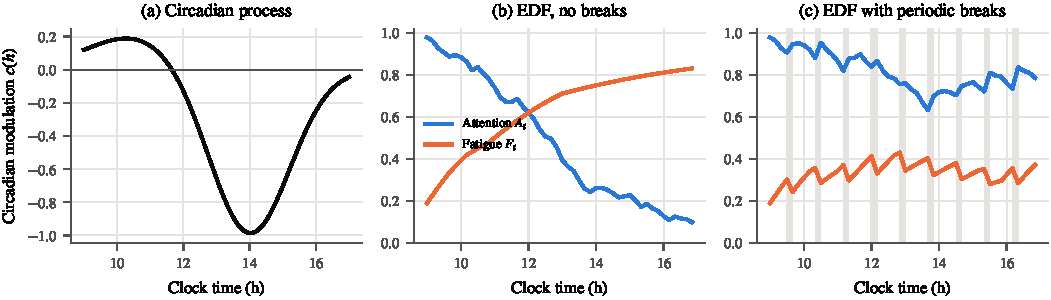
\includegraphics[width=\textwidth]{figures/fig_dynamics.pdf}
\caption{Simulator dynamics. (a) Circadian modulation $c(h)$ with a late-morning peak and post-lunch dip. (b) Effective attention and fatigue on one held-out test day under EDF without breaks. (c) The same day under EDF with a break after every four work slots (shaded bands mark breaks). Breaks keep attention high and fatigue low at the cost of working time.}
\label{fig:dynamics}
\end{figure}

\subsection{Observation model and partial observability}
The scheduler cannot observe $H_t$, $A_t$ or $F_t$. It receives noisy estimates
\begin{equation}
\tilde A_t=\mathrm{clip}(A_t+\sigma_o\epsilon^A_t,0,1),\qquad \tilde F_t=\mathrm{clip}(F_t+\sigma_o\epsilon^F_t,0,1),\qquad \epsilon^{A}_t,\epsilon^{F}_t\sim\mathcal N(0,1),
\label{eq:obs}
\end{equation}
with $\sigma_o=0.10$ in the nominal setting. These estimates stand in for wearable, ocular, behavioural or self-report estimators, whose errors are substantial in practice \cite{charles2019,borghini2014,hogervorst2014}. The full observation is the 13-dimensional vector
\begin{equation}
o_t=\Big[\tfrac{t}{T},\ \tilde A_t,\ \tilde F_t,\ \underbrace{\tfrac{n^e_t}{N},\ \tfrac{W^e_t}{20},\ \sigma^e_t,\ \tfrac{m^e_t}{N},\ \tfrac{\omega^e_t}{4}}_{\text{easy class}},\ \underbrace{\tfrac{n^h_t}{N},\ \tfrac{W^h_t}{20},\ \sigma^h_t,\ \tfrac{m^h_t}{N},\ \tfrac{\omega^h_t}{4}}_{\text{hard class}}\Big],
\label{eq:o}
\end{equation}
where, for each class, $n_t$ is the number of available unfinished tasks, $W_t$ their remaining work, $\sigma_t=\mathrm{clip}\big((\min_i D_i-t)/T,-1,1\big)$ the normalised slack of the most urgent task (1 if the class is empty), $m_t$ the number of overdue tasks, and $\omega_t$ the remaining work of the shortest task (0 if the class is empty). Unlike a binary completion vector, this summary is invariant to the number of tasks and exposes the deadline information that urgency-aware scheduling requires. The worker's true state and the future arrivals are hidden, so the decision problem is a POMDP $\langle\mathcal S,\mathcal A,P,R,\Omega,O,\gamma_{\mathrm{RL}}\rangle$ \cite{kaelbling1998}. Here $\mathcal S$ contains the full task set and $(H_t,F_t,t)$, $\Omega$ is the observation space of Eq.~\eqref{eq:o}, $O$ is given by Eq.~\eqref{eq:obs}, and $P$ by Eqs.~\eqref{eq:attention}--\eqref{eq:rho} together with the arrival process.

\subsection{Action space}
The agent chooses among five macro-actions,
\begin{equation}
\mathcal A=\{\textsc{easy},\ \textsc{hard},\ \textsc{edf},\ \textsc{spt},\ \textsc{break}\}.
\end{equation}
\textsc{easy} (\textsc{hard}) dispatches the available easy (hard) task with the earliest deadline, falling back to the other class if the chosen class is empty. \textsc{edf} and \textsc{spt} dispatch, across both classes, the task with the earliest deadline or the least remaining work. \textsc{break} allocates the slot to rest, and the worker also rests when no task is available. The first two actions let the agent regulate the cognitive \emph{intensity} of work relative to the worker's state. The two rule actions let it switch between urgency-driven and throughput-driven sequencing, in the spirit of DRL schedulers that select among dispatching rules \cite{luo2020,panzer2022}. This hybrid design has an important methodological consequence: every rule-based baseline in Section~\ref{sec:baselines} can be expressed as a policy over $\mathcal A$, so a learned policy is never handicapped relative to the baselines by its action space. Section~\ref{sec:component} reports an agent restricted to the intensity actions $\{\textsc{easy},\textsc{hard},\textsc{break}\}$ of the original formulation. The action space is independent of $N$, and tasks are preemptible at slot boundaries, which is common in knowledge work.

\subsection{Reward}
The per-slot reward combines task outcomes with cognitive terms:
\begin{equation}
r_t=\underbrace{\sum_{i\in\mathcal C_t}(1+d_i)\big[\mathbb 1(t+1\le D_i)+0.25\,\mathbb 1(t+1>D_i)\big]-0.5\,|\mathcal M_t|}_{r^{\text{task}}_t}\;+\;\mu A_{t+1}\;-\;\lambda F_{t+1},
\label{eq:reward}
\end{equation}
where $\mathcal C_t$ is the set of tasks completed in slot $t$, $\mathcal M_t$ is the set of tasks whose deadline expires unfinished at the end of slot $t$, $\mu=0.05$ and $\lambda=0.10$. Harder tasks are worth more, late completion retains a quarter of the value, and each missed deadline costs $0.5$. The attention and fatigue terms express the organisation's preference for sustainable work. Because such terms can change the optimal policy \cite{ng1999}, we (i) report reward-independent operational metrics (on-time rate, completion, fatigue exposure) alongside the return, (ii) train an agent with $\lambda=\mu=0$ to show that the learned behaviour is driven by the dynamics rather than by the reward terms, and (iii) sweep $\lambda$ to trace the productivity--fatigue Pareto front. The objective is to find a policy $\pi$ that maps observation histories to actions and maximises $\mathbb E_\pi\big[\sum_{t=0}^{T-1}\gamma_{\mathrm{RL}}^t r_t\big]$.

\begin{table}[t]
\centering
\caption{Nominal simulator parameters and their rationale.}
\label{tab:params}
\small
\begin{tabular}{p{4.3cm}lp{7.0cm}}
\toprule
Parameter & Value & Rationale / source \\
\midrule
Slots per day $T$, slot length $\Delta$ & 48, 10 min & 8-h workday; decision granularity of micro-breaks \cite{albulescu2022} \\
Tasks per day $N$ (initial / arriving) & 12 (6 / 6) & conditionally overloaded day; stochastic arrivals \\
Difficulty $d_i$, hard threshold & $\mathcal U[0.2,1]$, 0.6 & range of the original formulation \\
Work content $w_i$ & $1+2.5d_i$ units & 15--35 min at full capacity \\
Relative slack $s_i$ & $\mathcal U[0.3,1]$ & range of the original formulation \\
Attention depletion $\alpha$, fatigue coupling $\phi$ & 0.02, 0.5 & vigilance decrement over hours of work \cite{warm2008,thomson2015} \\
Attention recovery $\beta$ & 0.30 per slot & break benefits \cite{ariga2011,albulescu2022} \\
Circadian amplitude $\gamma$ & 0.15 & post-lunch dip \cite{monk2005,schmidt2007} \\
Fatigue accumulation $\delta$, recovery $\eta$ & 0.05, 0.20 & exponential fatigue--recovery \cite{jaber2010,jaber2013} \\
Fatigue throughput penalty $\kappa$ & 0.5 & performance loss under fatigue \cite{boksem2008,vandongen2003} \\
Process / observation noise $\sigma_p,\sigma_o$ & 0.02, 0.10 & variability; sensor error \cite{charles2019,hogervorst2014} \\
Reward weights $\mu,\lambda$ & 0.05, 0.10 & swept in Section~\ref{sec:pareto} \\
\bottomrule
\end{tabular}
\end{table}
